\documentclass[output=paper]{langsci/langscibook}
\author{M. Rita Manzini\affiliation{University of Florence}\and Leonardo M. Savoia\affiliation{University of Florence}}
\title{Person splits in Romance: Implications for parameter theory}

% \chapterDOI %will be filled in at production

\abstract{This contribution addresses person splits in which 1/2P and 3P, or 1P
    and 2P systematically differ from one another with respect to the core
    grammar properties of case and agreement, giving raise to parametric
    variation. We consider two case studies from \ili{Romance} varieties. The
    first one concerns 1/2P object \isi{clitics} which, in \ili{Italian} like
    in other \ili{Romance} languages, have a simplified morphology with respect
    to 3P \isi{clitics}, namely a single gender- and case-neutral object form,
    as opposed to the accusative\is{accusative case} vs. dative\is{dative case}
    distinction, and the gender distinctions found in 3P. Moreover, 1/2P
    \isi{clitics} only optionally trigger perfect participle (\emph{v})
    agreement, otherwise obligatory with 3P accusative\is{accusative case}
    \isi{clitics}. We argue that these behaviors correspond to a core syntax
    phenomenon, whereby 1/2P \isi{clitics} trigger DOM, which in the
    \ili{Romance} languages takes the form of obliquization. The fact that 1/2P
    \isi{clitics} are DOM\is{differential object marking} obliques explains
    their specialized behavior in comparison with 3P \isi{clitics}. The second
    case study has to do with partial pro-drop\is{null subjects} patterns in
    Northern \ili{Italian} dialects involving the 1P vs. 2P split, interacting
    with the Externalization process and the Recoverability principle. We show
    that the (micro)parameters regulating the distribution of subject
    \isi{clitics} are best seen as a reflex of macrocategories of grammar.
    Finally, we compare our approach with the literature on these phenomena
    \parencite{CardinalettiRepetti2008,Calabrese2008} and with the ReCoS
    parametric theory of Ian Roberts and his collaborators, discussing their
different explanatory capabilities and results.}

\maketitle

\begin{document}\glsresetall

\section{Introduction}\label{sec:06.1}

Our focus in this contribution is person splits, by which we mean interactions
between pronouns and syntactic rules and relations such as \isi{Agree}, Case,
etc. in which 1/2P and 3P, or 1P and 2P, are seen to systematically differ from
one another. We provide two case studies from \ili{Romance}
varieties.\footnote{Though our focus is on Northern \ili{Italian} dialects
    (\Cref{sec:06.2}) and on Standard \ili{Italian} (\Cref{sec:06.1}), the
    title refers to \ili{Romance} varieties, in that the database of
\citet{ManziniSavoia2005}, which we use in particular in \Cref{sec:06.2},
includes \ili{Occitan}, Franco-Provençal and \ili{Ladin} (Rhaeto-Romance) dialects, spoken
within the borders of Italy and Switzerland.} In \Cref{sec:06.2} we argue
that partial pro-drop\is{null subjects} patterns in Northern \ili{Italian} dialects involve the 1P vs.\
2P split, interacting with the Externalization process and the Recoverability
principle. Though the possible parametric values individuate a \isi{microvariation}
set (including only subject \isi{clitics}), the \isi{parameters} are best identified with
the categorial splits themselves (such as 1/2P vs.\ 3P etc.), which involve
macrocategories of grammar.

In this section, we concentrate on object \isi{clitics} in Standard \ili{Italian},
henceforth \ili{Italian}. 1/2P object \isi{clitics} have a simplified morphology (a single
object form, gender neutral) with respect to 3P \isi{clitics} (encompassing the
accusative vs.\ dative\is{dative case} distinction and gender distinctions). They also only
optionally trigger perfect participle (\emph{v}) agreement. We argue that these
behaviours do not involve low-level morphological readjustments – but
correspond to core syntactic phenomena. In this respect, we reject not just
descriptive accounts, but also accounts that require an independent
morphological component within formal models.

Several properties distinguish 1/2P \isi{clitics} from 3P \isi{clitics} in \ili{Romance}, which
for ease of exposition we will illustrate with just one language, namely
Italian. Leaving aside the locative/instrumental \emph{ci}, the genitive\is{genitive case}
\emph{ne} and the middle-reflexive \emph{si}, the inventory of \ili{Italian} \isi{clitics}
is as in \tabref{tab:06.1}. What is immediately evident from the table is that
3P \isi{clitics} are differentiated by gender (masculine/feminine) and by case
(accusative/dative) – but 1/2P are insensitive to either distinction.

\begin{table}
    \begin{tabular}{llllll}
    \lsptoprule
                 & \Acc.\M & \Acc.\glossF{} &           & \Dat.\M     & \Dat.\glossF{}\\\midrule
    \Fsg       &           &           & \emph{mi} &               & \\
    \Ssg       &           &           & \emph{ti} &               & \\
    \Tsg       & \emph{lo} & \emph{la} &           & \emph{gli}    & \emph{le}\\
    \Fpl       &           &           & \emph{ci} &               & \\
    \Spl       &           &           & \emph{vi} &               & \\
    \Tpl       & \emph{li} & \emph{le} &           & \emph{(loro)} & \emph{(loro)}\\
    \lspbottomrule
    \end{tabular}
    \caption{Italian accusative\is{accusative case} and dative\is{dative case}
    clitics}\label{tab:06.1}
\end{table}

The classical approach to asymmetries like those in \REF{ex:06.1} is to
postulate a single underlying phi-features\is{φ-features} and case system, namely a system
rich enough to be able to account for 3P – and to assume that morphological
mechanisms (perhaps impoverishment\is{impoverishment} and underspecification,
in the way of \isi{Distributed Morphology}) are responsible for the surface
syncretisms observed in 1/2P. However, there is a third phenomenon with respect
to which 1/2P and 3P differ, which does not directly involve the morphology of
the \isi{clitics}, but rather their syntactic behavior. As shown by
\citet{Kayne1989}, in \ili{Italian} (and \ili{French}, etc.) perfect
participles \isi{Agree} with D(P) complements moved to their left, hence with
accusative\is{accusative case} \isi{clitics}. Dative\is{dative case} clitics do
not \isi{Agree}, even if they are associated with gender features in normative
\ili{Italian}. We may assume that this is due to the fact that they are
embedded under an oblique case. The relevant contrasts with 3P \isi{clitics}
are illustrated in \REF{ex:06.1}.

\ea\label{ex:06.1} \ili{Italian}
    \ea[]{
	\gll    Lo / la / li / le     ha aiutat-o / aiutat-a / aiutat-i / aiutat-e\\
    him {} her {} them-\M{} {} them-\glossF{}  he.has helped-\M.\Sg{} {}
    talked-\glossF.\Sg{} {} talked-\M.\Pl{} {} talked-\glossF.\Pl{}\\
    \glt    ‘He helped him / her / them’}
    \ex[*]{
	\gll    la / li / le       ha   aiutat-o\\
            her {} them-\M{} {} them-\glossF{}  he.has   helped-\M.\Sg{}\\
    \glt    ‘He helped her / them’}
    \ex[]{
	\gll    Gli / le       ha   parlat-o / *parlat-a\\
    to.him {} to.her  he.has   talked-\M.\Sg{} {} \hphantom{*}talked-\glossF.\Sg{}\\
    \glt     ‘He talked to him / her’}
    \ex[]{
	\gll  Ha   loro       parlat-o / *parlat-i / *parlat-e\\
    he.has   to.him/to.her  talked-\M.\Sg{} {} \hphantom{*}talked-\M.\Pl{} {}
    \hphantom{*}talked-\glossF.\Pl{}\\
    \glt     ‘He talked to him / her’}
    \z
\z

Surprisingly, notionally accusative\is{accusative case} 1/2P \isi{clitics} may
not \isi{Agree} in either gen\-der or number, as in (\ref{ex:06.2}a),
paralleling the dative\is{dative case} clitic in (\ref{ex:06.2}c).
Agreement of the 1/2P clitic with the perfect participle, as seen in
(\ref{ex:06.2}b), remains possible, but it is optional. Free alternations
of this type are standardly seen as pointing to the existence of two slightly
different grammars. In the first one, 1/2P \isi{clitics} \isi{Agree} with the
perfect participle; in the alternative grammar they do not. If two slightly
different languages are involved in the free alternation of agreeing and
non-agreeing participles in \REF{ex:06.3}, we expect there to be languages
where only agreement is allowed and languages where only invariable participial
forms are. Indeed there are many \ili{Italian} varieties where 1/2P never
trigger agreement (contrary to 3P forms), as documented by
\textcite[§5.1.2]{ManziniSavoia2005}.

\ea\label{ex:06.2} \ili{Italian}
   	\ea
	\gll    Mi / ti / ci / vi  ha aiutato\\
            me {} you {} us {} you.\Pl{}  he.has  helped-\M.\Sg{}\\
	\glt    ‘He helped me / you / us’
 	\ex
	\gll    Mi / ti      ha   aiutata\\
            me {} you   he.has   helped-\glossF.\Sg{}\\
	\glt    ‘He helped me / you’
 	\ex
	\gll    Ci / vi       ha   aiutati / aiutate\\
            us {} you.\Pl{}  he.has helped-\M.\Pl{} {} helped-\glossF.\Pl{}\\
	\glt    ‘He helped us / you’
    \ex
    \gll    Mi / ti / ci / vi    ha parlato / *parlata / *parlati / *parlate\\
    to.me {} to.you {} to.us {} to.you.\Pl{} he.has talked-\M.\Sg{} {}
    \hphantom{*}talked-\glossF.\Sg{} {} \hphantom{*}talked-\M.\Pl{} {}
    \hphantom{*}talked-\glossF.\Pl{}\\
    \glt    ‘He talked to me / you / us’
    \z
\z

It is true that, as we have noticed at the beginning, 1/2P pronouns lack
nominal class features, but they have overt number properties. Therefore,
relating optionality in agreement to the lack of (overt) morphological features
is not immediately possible. What is more, under a morphological analysis, we
would expect 1/2P to always display optional agreement, while agreement is
clearly obligatory in subject contexts, as in \REF{ex:06.3}. The same
incidentally is true in Northern \ili{Italian} dialects where 1/2P subjects are
obligatorily realized as \isi{clitics}. This forces the view that the optionality of
1/2P object agreement\is{agreement!object agreement} depends not on the lexical content of the 1/2P forms, but
rather on their structure of embedding.

\ea%3
    \label{ex:06.3}
    \ea
	\gll    (Io\textsubscript{\glossF})   sono  arrivata / *arrivato\\
            \hphantom{(}I.\glossF{} am  arrived-\glossF.\Sg{} {} \hphantom{*}arrived-\M.\Sg{}\\
	\glt    ‘I have arrived’
 	\ex
    \gll    (Noi) siamo arrivati / arrivate / *arrivato\\
    \hphantom{(}we  are   arrived-\M.\Pl{} {} arrived-\glossF.\Pl{} {}
    \hphantom{*}arrived-\M.\Sg{}\\
    \glt    ‘We have arrived’
    \z
\z

The alternative option, taken by \citet{ManziniSavoia2005} and \citet{Kayne2010},
is embedding the analysis of \isi{clitics} firmly within core syntax, including their
apparently idiosyncratic syncretisms. As \citet[144]{Kayne2010} argues,
“syncretism of the sort under consideration is nothing other than a particular
kind of syntactic ambiguity”. Specifically, addressing the
1\textsuperscript{st} pronoun plural \emph{ci} (syncretic with locative) he
proposes that “it is not that \emph{ci} has multiple possible values. Rather,
\emph{ci}, the same \emph{ci}, is compatible in \ili{Italian} with a certain range of
syntactic contexts, … a silent PLACE, … a silent \Fpl{}”, where silent
constituents are constituents grammatically represented but not pronounced.
\citet{ManziniSavoia2005}, \citet{Manzini2012}, and \citet{ManFra2016}
provide partial discussions of the range of empirical data that interests us
here, which we will pursue in a more systematic manner in what follows.

\subsection{Clitics and Case}\label{sec:06.1.1}

We pointed to three respects in which 1/2P objects differ from 3P objects. Two
of them involve relational notions, namely case and agreement. Before we turn
to them, let us consider the different phi-features\is{φ-features} make-up displayed by the
two series of pronouns. The absence of nominal class endings (gender) on 1/2P
clitics is a pan-Romance characteristic. In fact, according to
\citet[194]{Siewierska2004}, “gender oppositions are characteristic of third
rather than first or second person. Of the 133 languages in the sample (33\%)
which have gender in their independent person forms, 129 (97\%) have gender in
the third person as opposed to 24 (18\%) in the second and three in the first
(3\%)”.\footnote{We thank Ludovico Franco for research and discussion
on this point.} Furthermore 1/2P forms are differentiated for number via
their lexical basis. Thus even in \ili{Romance} languages in which number is factored
away from nominal class and lexicalized by a specialized \emph{-s} ending, it
is impossible to have 1\textsuperscript{st} plural formed by adding -\emph{s}
to 1\textsuperscript{st} singular. This is not necessarily a consequence of the
absence of gender inflections. For instance, Sardinian varieties which present
a dative\is{dative case} singular form not inflected for gender, of the type
\emph{li} ‘to him/her’, also regularly pluralize it as \emph{li-s} ‘to them’
(\citealt{ManziniSavoia2005}).

By contrast, the generalization holds that in \ili{Romance} languages 3P \isi{clitics} have
an internal structure comparable to that of lexical nouns. Simplifying
somewhat, the consensus in the literature is that at least two functional
projections are needed for Ns – corresponding roughly to gender and number. In
homage to the cross-linguistic comparison with \ili{Bantu} languages, the lower
category is often labelled Class, the higher category is Num
\citep{Picallo2008}, i.e.\ [[${\sqrt{}}$ Class] Num].  Extra complexity arises in
\ili{Indo-European} languages from the fact that there is no one-to-one mapping
between the content of Class, which enters agreement with determiners and
modifiers of N, and the inflections immediately following the root. We
tentatively assign the inflectional vowel of \ili{Italian} to an Infl position~–
which embeds both the root and the Class node. Transposed to the analysis of
singular 3P \isi{clitics}, this yields structures like \REF{ex:06.4}.

\ea%4
    \label{ex:06.4}
    \begin{tikzpicture}[baseline=(root.base)]

        \Tree 	[.\node(root){D};
                    [.D
                        {D\\\emph{l-}}
                        {Class\\{}[masc]/[fem]}
                    ]
                    {Infl\\\emph{-o}/\emph{-a}}
                ]

    \end{tikzpicture}
\z

Languages like \ili{Spanish} have an independent lexicalization for the plural,\linebreak
namely \emph{-s}; in \ili{Italian} however pluralization is obtained by a change of
the inflectional vowel. We may suppose that the plural 3P \isi{clitics}, namely
\emph{li/le}, have the structure in \REF{ex:06.5}, where the plural property
is associated with the Class node. Note that this is in keeping with current
ideas about Num not being a quantifier – but rather a divisibility predicate
\citep{Borer2005}.

\ea%5
    \label{ex:06.5}
    \begin{tikzpicture}[baseline=(root.base)]
        \Tree 	[.\node(root){D};
                    [.D
                        {D\\\emph{l-}}
                        {Class\\{}[fem]/[masc]\\{}[\Pl]}
                    ]
                    {Infl\\\emph{-e}/\emph{-i}}
                ]
    \end{tikzpicture}
\z

The morphological structures in (\ref{ex:06.4}--\ref{ex:06.5}) map to a
compositional semantics, essentially as outlined by \citet[221]{Kratzer2009}:

\begin{quote}
the alleged “3rd person” features are in fact gender features, a variety of
descriptive feature ... If [a descriptive feature] is to grow into a pronoun,
it has to combine with a feature [def] that turns it into a definite
description. If [def] is the familiar feature that can also be pronounced as a
definite determiner in certain configurations, it should head its own
functional projection, hence be a D. It would then not originate in the same
feature set as descriptive features, which are nominal, hence Ns.
\end{quote}

\noindent In this
perspective, the pan-Romance (near-universal) fact that 1/2P forms are not
associated with gender morphology, far from being a morphological syncretism or
other quirk of pronunciation, corresponds to a potentially interesting
\mbox{(morpho)}syntactic generalization – namely that 1/2P are pure deictic forms,
deprived of predicative restrictions, even as elementary as Class (gender,
countability).

A notable characteristic of \ili{Italian} 1/2P \isi{clitics}, apart from the lack of
nominal class inflections, is the absence of case differentiations or, if one
wishes, the accusative/dative syncretism – which is also replicated by many
languages (e.g.\ \ili{French}, \ili{Spanish}, \ili{Albanian}), though not by all (e.g.\ \ili{Romanian},
\ili{Greek}). In fact, in \ili{Italian} \REF{ex:06.2}, the \emph{m-i,} \emph{t-i} 1/2P
person forms have the same \emph{-i} inflection as the 3P dative\is{dative case} \emph{gl-i}.
This inflection contrasts with that of the accusative\is{accusative case} in \REF{ex:06.1},
corresponding to gender morphology (\emph{-o, -a, -i, -e}).\footnote{\emph{-i}
    is the Latin inflection of the dative\is{dative case} singular (in all declension classes
    excepting the II), also syncretic with the genitive\is{genitive case} (in the I class).  Note
    further that though in \tabref{tab:06.1}, we have illustrated normative
Italian, in colloquial \ili{Italian} there is a single dative\is{dative case} form for masculine and
feminine, singular and plural, corresponding to \emph{gli} (\emph{l-}
definiteness base + -\emph{i} inflection).} Now, obliquization and specifically
dativization of highly ranked referents normally characterized \gls{DOM}\is{differential object marking} in
\ili{Indo-European} languages (\citealt{ManFra2016}).  Specifically in \ili{Romance},
\gls{DOM} marking of lexical DPs generally takes the form of the preposition
\emph{a} ‘to’ (in Ibero-Romance, in Southern \ili{Italian}
dialects).\is{DOM|see{differential object marking}}

At the basis of \gls{DOM}\is{differential object marking} is the fact that in many languages, case assignment depends
on the referential content of the argument DPs. This is often described in
terms of an \isi{animacy} hierarchy. The classical discussion by
\citet[85--86]{Dixon1979} is based on the “potentiality of agency” scale, i.e\
1\textsuperscript{st} person $<$ 2\textsuperscript{nd} person $<$
3\textsuperscript{rd} person $<$ proper name $<$ human $<$ animate $<$ inanimate.
According to Dixon, 

\begin{quote}
it is plainly most natural and economical to “mark” a
participant when it is in an unaccustomed role\dots{} A number of languages have
split case-marking systems exactly on this principle: an ergative\is{ergative case} case is used
with NPs from the right-hand end, up to some point in the middle of the
hierarchy, and an accusative\is{accusative case} case from that point on, over to the extreme left
of the hierarchy\dots{} Though the phenomenon is often referred to under the
heading of split ergativity, it is evident that in the typological continuum it
touches what we may call split accusativity.
\end{quote}

\noindent Similarly, using a different
terminology, \citet[473]{Aissen2003} states that “the factors that favor
differential subject marking will be the mirror image of those that favor DOM”.

The overt dative\is{dative case} morphology of \gls{DOM}\is{differential object marking} objects suggests that these forms are not
directly embedded as the internal argument of the event. Rather, their
embedding requires the presence of a case layer, the dative\is{dative case}, dedicated to the
expression of possessors. We follow \citet[170]{BeldenDik1997} in
characterizing the possession relation in terms of zonal inclusion, i.e.
“[e]ntities have various zones associated with them, such that an object or
eventuality may be included in a zone associated with an entity without being
physically contained in that entity”. Following \citet{Manzini2012}, we label
the dative\is{dative case} case, carrying the relational inclusion content, as ${\subseteq}$.

In these terms, the structure of embedding of \emph{mi/ti} in \REF{ex:06.2}
remains constant despite the fact that two different structures of embedding
are implied by the predicates \emph{aiutare} ‘help’ and \emph{parlare} ‘speak
(to)’ with 3P \isi{clitics} in \REF{ex:06.1}. In the structure in \REF{ex:06.6} we
propose that the two arguments of ${\subseteq}$ are the 1/2P clitic and – we
assume – the event itself, adopting and adapting in this respect an idea of
the applicative literature \citep{Pylkkanen2008}.

\ea%6
    \label{ex:06.6}
    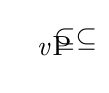
\begin{tikzpicture}[baseline=(root.base)]

        \Tree 	[.\node(root){\emph{v}P};
                    {\emph{v}\\\Caus}
                    [.VP
                        {V\\\emph{aiuta-}\\\emph{parla-}}
                        [.$\subseteq$P
                            {1/2P\\\emph{m}}
                            {$\subseteq$\\\emph{i}}
                        ]
                    ]
                ]

    \end{tikzpicture}
\z

Intuitively, transitive predicates can be paraphrased by an elementary
predicate associated with an eventive name. Thus \emph{aiutare} ‘help’
alternates with \emph{dare} \emph{aiuto} \emph{a} ‘give help to’.
\citet{HaleKeyser1993}, \citet{Chomsky1995} formalize this intuition about the
complex nature of transitive predicates by assuming that they result from the
incorporation of an elementary state/event into a transitivizing (typically
causative) predicate. Within such a conceptual framework it becomes clearer
what we mean when we say that in \REF{ex:06.6}, ${\subseteq}$ takes as its
arguments the 1/2P pronoun and an elementary state/event. In other words,
\REF{ex:06.6} can be informally rendered as ‘He caused me to have help/talk’.
We claim that the 1/2P pronoun in \REF{ex:06.6} is introduced as a possessor,
taking in its “zonal inclusion” domain an elementary event – for instance
\emph{aiuto} ‘help’. By contrast, 3P complements of \emph{aiutare} ‘help’ (or
rather ‘cause help’) are embedded in a canonical transitive (causative)
structure comprising a nominative\is{nominative case} agent and an accusative\is{accusative case} theme. The fact 3P
arguments of \emph{parlare} ‘talk (to)’ require the ${\subseteq}$ embedding
must be considered a lexically governed alternation (subject to considerable
cross-linguistic variation, see \citealt{Svenonius2002}).

\citet{ManFra2016} discuss potential problems for the present analysis
in some detail. Specifically, the 1/2P argument of \emph{aiutare} ‘help’ raises
to the nominative\is{nominative case} position in the passive\is{passive}, while that of \emph{parlare} ‘talk
(to)’ does not, as in (\ref{ex:06.7}a) vs.\ (\ref{ex:06.7}b). The contrast in
passivization is traditionally explained by the assumption that underlying
cases are identical for 1/2P and 3P, though 1/2P are morphologically syncretic
between dative\is{dative case} and accusative\is{accusative case}. Thus the accusative\is{accusative case} object of \emph{aiutare}
‘help’ can be passivized independently of whether it is 1/2P or 3P, while that
of \emph{parlare} ‘talk (to)’ cannot. Therefore the possible way to passivize
\emph{parlare} ‘talk (to)’ is an impersonal passive\is{passive}, as in
(\ref{ex:06.7}b$'$).

\ea%7
\label{ex:06.7} \ili{Italian}
    \ea[]{
	\gll    Sono stato aiutato\\
            I.am been helped\\
    \glt    ‘I was helped’}
    \ex[*]{
	\gll    Sono stato parlato\\
            I.am  been spoken\\
    \glt    ‘I was spoken to’}
    \exi{b$'$.}[]{
	\gll    Mi   è   stato parlato (di te)\\
            to.me  it.is  been talked \hphantom{(}of you\\
    \glt    ‘It was talked to me (about you)’}
    \z
\z

\citet{ManFra2016} propose a different explanation. They argue that the dative\is{dative case}
case with \emph{parlare} ‘talk (to)’ is inherent, in the sense of
\citet{Chomsky1986}, i.e.\ it is selected by the verb. Under passive\is{passive}, inherent
dative case must be preserved, yielding an impersonal passive\is{passive}, as in
(\ref{ex:06.7}b$'$) but barring \isi{raising} to nominative\is{nominative case}
position as in (\ref{ex:06.7}b). On the contrary, the dative\is{dative case} case with
\emph{aiutare} ‘help’ and 1/2P objects is structural, since it depends not on
the selection properties of the verb, but on the DOM\is{differential object marking} configuration. Passive
voids the context for the application of DOM, since the internal argument is
raised out of its VP-internal position to [Spec, IP].  Therefore, no dative\is{dative case}
need be present in the derivation and sentences like (\ref{ex:06.7}a) are
well-formed.

Before turning to agreement, it is worth mentioning that independent evidence
for the presence of 1/2P vs.\ 3P splits in \ili{Romance} \gls{DOM}\is{differential object marking} comes also from
full pronouns – though it can only be briefly reviewed here. The standardly
recognized manifestation of \gls{DOM}\is{differential object marking} in the \ili{Romance} languages is the so-called
prepositional accusative\is{accusative case}, whereby in a large number of \ili{Romance} varieties
(Ibero-Romance, Central and Southern \ili{Italian} dialects, Romansh, Corsican,
Sardinian, \ili{Romanian}) highly ranked objects are introduced by a preposition
(with or without \isi{clitic doubling}), most often \emph{a}. The best known and most
frequently attested pattern has \gls{DOM}\is{differential object marking} associated with definite/animate DPs,
as in Standard \ili{Spanish} (see \citealt{Aissen2003} for a typological survey,
\citealt{vHeuKai2011} for a corpus study). However, as illustrated
\textcite[§4.9]{ManziniSavoia2005}, \citet{DAlessandro2015}, other splits along the
descriptive animacy/definiteness hierarchies are attested by \ili{Italian} varieties.
What is relevant for present purposes is that in some Center-South \ili{Italian}
varieties only 1/2P internal arguments require DOM, as in (\ref{ex:06.8}a).
3P pronouns and kinship terms (essentially functioning as proper names) undergo
ordinary (bare) embedding, as in (\ref{ex:06.8}b).\footnote{Other varieties
    displaying the same pattern are Cagnano Amiterno (Abruzzi) and Borbona
    (Lazio); optionality of \gls{DOM}\is{differential object marking} in the 3P characterizes a few more
    dialects in the corpus, specifically Avigliano Umbro (Umbria), Torricella
    Peligna (Abruzzi), Canosa Sannita (Abruzzi).  In fact, in contexts
    involving 1/2P pronouns, or in any event pronouns, DOM\is{differential object marking} and \isi{clitic doubling}
    can also surface in Northern \ili{Italian}.  In (i) we reproduce an example from
    Trieste (an anonymous reviewer suggests data from the dialectologically
    close variety of Padua).

\begin{exe}
    \exi{(i)} Trieste, Venezia Giulia \parencite[548]{Ursini1988}\\
    \gll    el   te   ga bastonado   a ti\\
            he   you   has beaten \textsc{dom} you\\
    \glt    ‘He beat you up’
\end{exe}\label{fn:06.4}}

\ea%8
    \label{ex:06.8} \ili{Italian} Colledimacine (Abruzzi, \citealt{ManziniSavoia2005}: 505)
    \ea
	\gll    a   camatə   a mme / a nnu\\
            he.has  called  \textsc{dom} me {} \textsc{dom} us\\
	\glt    ‘He called me / us’
 	\ex
	\gll    a   camatə   frattə tiə / kwiʎʎə\\
            he.has  called   brother yours {} him\\
	\glt    ‘He called him / my brother’
    \z
\z

Importantly, though the evidence from \ili{Italian} 1/2P \isi{clitics} reviewed
would traditionally be treated in terms of morphological syncretism, there is
no question that facts like \REF{ex:06.8} are syntactic.

\subsection{Clitics and Agree}\label{sec:06.1.2}

Let us then turn to agreement. Consider first 3P \isi{clitics}. Under
\citeauthor{Chomsky2000}'s (\citeyear{Chomsky2000,Chomsky2001}) model of
\isi{Agree}, we may say that transitive verbs (i.e.\ verbs with an external
argument and a \emph{v} structural layer) include a probe on \emph{v}, which
attracts the closest argument (by Minimal Search), namely the object of V.
\isi{Agree} (i.e.\ Match/Identity) then goes through, yielding
(\ref{ex:06.9}a); for the sake of exposition we have assumed that the
clitic has a base position inside the VP. Otherwise, the perfect participle
turns up inflected with the invariable masculine singular ending, as in
(\ref{ex:06.9}b). The traditional assumption in this respect is that some
sort of morphological default repairs the lack of syntactic agreement.

\ea%9
    \label{ex:06.9}
    \ea {}[\textsubscript{\emph{v}P} \emph{aiutata} [\textsubscript{D} \emph{la}]]
    \ex {}[\textsubscript{\emph{v}P} \emph{parlato} [\textsubscript{${\subseteq}$} [\textsubscript{D} \emph{gli/le}]]]\\
    \z
\z

For ease of exposition, we have assumed that the perfect participle is an
unanalyzed unit, associated with a probe in the form of a feature matrix,
essentially as in \citet{Chomsky1995}. In reality, the perfect participle
consists of a lexical base (inclusive of a so-called thematic, or inflectional
class, vowel, which will be disregarded here), followed by a perfect ending
\emph{-t}, followed in turn by a suffix containing gender and number
information (-\emph{o,} \emph{-a,} \emph{-i,} \emph{-e}), as in
\REF{ex:06.10}. The φ constituent is presumably to be identified
with the agreement probe.

\ea%10
    \label{ex:06.10}
    \begin{tikzpicture}[baseline, baseline=(root.base)]

        \Tree 	[.\node(root){V};
                    [.V
                        {$\sqrt{\hphantom{x}}$\\\emph{aiuta}}
                        {V\\\emph{-t}}
                    ]
                    {φ\\\emph{-o}/\emph{-a}/\emph{-i}/\emph{-e}}
                ]

    \end{tikzpicture}
\z

Classical theories of null subjects hold the view that the finite inflection of
languages like \ili{Italian} is pronominal-like \citep{Rizzi:1982}, hence it represents a
lexicalization of the subject. In fact, in some models the \emph{pro} empty
category is dispensed with altogether (\citealt{Borer1986} for an early
statement, \citealt{ManziniSavoia2005,ManziniSavoia2007}). Suppose we generalize this idea
to all agreement inflections. The perfect participle inflection, seen in
Italian \REF{ex:06.9}, will be construed as an elementary lexicalization of
the internal argument within the morphological structure of the verb, as
schematized in \REF{ex:06.10}. Classical theories of pro-drop\is{null subjects} hold the view
that the finite inflection of languages like \ili{Italian} is pronominal-like
\citep{Rizzi:1982}; in fact, some models treat it as satisfying the
\glsunset{EPP}\gls{EPP}, so that
the pro empty category becomes redundant \parencite{Borer1986,ManziniSavoia2005,ManziniSavoia2007}. Suppose we generalize this idea to all
agreement inflections. The perfect participle inflection will then be construed
as an elementary lexicalization of the internal argument, as schematized in
\REF{ex:06.11}.

\ea%11
    \label{ex:06.11}
    \begin{tikzpicture}[baseline=(root.base)]
        \Tree 	[.\node(root){V};
                    [.V
                        {$\sqrt{\hphantom{x}}$\\\emph{aiuta}\textsubscript{λx}}
                        {V\\\emph{-t}}
                    ]
                    {φ\\\emph{-o}/\emph{-a}/\emph{-i}/\emph{-e}\textsubscript{x}}
                ]
    \end{tikzpicture}
\z

In \REF{ex:06.11}, the φ constituent endowed with gender and number
(i.e.\ nominal class) specifications needs a 1/2P or D closure in order to
achieve referential status. This can only be obtained via the application of
\isi{Agree}. According to \citet[122]{Chomsky2000} “the simplest assumptions
for the probe--goal system” are formulated as in \REF{ex:06.12}. Matching,
namely feature identity according to (\ref{ex:06.12}a), “is a relation that
holds of a probe P and a goal G. Not every matching pair induces \isi{Agree}.
To do so, G must (at least) be in the domain D(P) of P”, defined as in
(\ref{ex:06.12}b).  Furthermore, “a matching feature G is closest to P if there
is no G' in D(P) matching P such that G is in D(G')” as in (\ref{ex:06.12}c).

\ea%12
    \label{ex:06.12} \textcite[122]{Chomsky2000}
    \ea Matching is feature identity.
	\ex D(P) is the sister of P.
    \ex Locality reduces to closest c-command.
    \z
\z

Our proposal (see also
\citealt{ManziniSavoia2005,ManziniSavoia2007,ManSav2011}) holds on to
these “simplest assumptions”, but revises their standard implementation, in
keeping with the need to interweave morphological and syntactic analysis.
Specifically, we may expand the schematic structure in (\ref{ex:06.9}a) as in
\REF{ex:06.13}. We translate the classical idea that φ features\is{φ-features} percolate to
the head level \emph{v} by assuming that \isi{labelling} creates a (\emph{v}, φ)
projection. At this point \isi{Agree} proceeds along the lines in
\REF{ex:06.12} creating a pair ordered by c-command and obeying locality,
normally taken to be (\emph{aiutata}, \emph{la}). We may equally, and more
perspicuously, pare the \isi{Agree} sequence down to (-\emph{a,} \emph{-a}).

\ea%13
    \label{ex:06.13}
    \begin{tikzpicture}[baseline=(root.base)]

        \Tree 	[.\node(root){\emph{v}P};
                    [.{(\emph{v}, φ)}
                        {\vphantom{V}\emph{v}\\\emph{aiutat}}
                        {\vphantom{V}φ\\\emph{-a}}
                    ]
                    [.VP
                        {V\\\sout{aiutata}}
                        [.{(D, φ)}
                            {D\\\emph{l}}
                            {φ\\\emph{-a}}
                        ]
                    ]
                ]

    \end{tikzpicture}
\z

We know that in \citeauthor{Chomsky2000}'s (\citeyear{Chomsky2000,Chomsky2001})
conception, \isi{Agree} is a matter of deleting the uninterpretable features of
the probe, with the result that a single copy of an agreement pair survives,
namely the interpretable copy of the goal. But this is simply a technical
implementation. One may keep closer to the morphological reality of agreement
and assume that agreement is a matter of feature unification. Thus the
agreement pair for \REF{ex:06.13} unifies the feminine features instantiated
by the \emph{-a} inflections of \emph{v} and D. As a result, the D features
morphologically instantiated by \emph{l-} provide the necessary and sufficient
referential closure for the internal argument of \emph{aiutare} ‘help’. In this
perspective, the satisfaction of Full Interpretation at the \gls{CI} interface
depends on the fact that the operation of \isi{Agree} creates an equivalence
set, interpreted as a single argument with multiple occurrences (what
\citealt{ManziniSavoia2007} call agreement chains).

Let us then consider the 3P non-agreeing pattern in (\ref{ex:06.9}b). The
internal structure of the perfect participle is as already indicated in
\REF{ex:06.9}, except that \emph{parlare} ‘speak (to)’ does not introduce an
internal argument. Rather, it selects the dative\is{dative case} preposition or case, i.e.\ an
element with (${\subseteq}$) relational content, introducing a possessor. As a
consequence, the φ node is externalized by the invariable \emph{-o}
ending, as in \REF{ex:06.14}; the latter could be the realization of an empty
φ node, i.e.\ what is traditionally called a default.\footnote{In a less
    stipulative way, in the absence of an internal argument, we could take the
    φ node to realize the abstract event argument. Note that in \ili{Romance}
    languages where productive neuter gender is available (Central \ili{Italian}
dialects, \citealt{ManziniSavoia2005,ManziniSavoia2017}), the latter is
associated with mass and eventive contents and also with invariable perfect
participles.\label{fn:06.5}}

\ea%14
    \label{ex:06.14}
    \begin{tikzpicture}[baseline=(root.base)]

        \Tree 	[.\node(root){V};
                    [.V
                        {$\sqrt{\hphantom{x}}$\\\emph{parla}}
                        {V\\\emph{-t}}
                    ]
                    {φ\\\emph{-o}}
                ]

    \end{tikzpicture}
\z

At this point, we are in a position to consider the crucial 1/2P data.
Specifically, with \emph{aiutare} ‘help’ two alternatives are possible. In
present terms, the first alternative consists in the partial saturation of the
internal argument of the participle by a gender and number inflection, as in
\REF{ex:06.14-2}. The φ probe can be matched with the 1/2P content as
a goal, creating an agreement pair. The operation requires that the 1/2P
constituent is visible despite the presence of ${\subseteq}$ oblique
morphology; in other words the ${\subseteq}$ case morphology must be
transparent. We already suggested in the discussion surrounding
\REF{ex:06.13} that the right way to think about agreement pairs is not in
terms of feature deletion (à la Chomsky), but rather of feature unification.
Hence the descriptive gender and number properties of the \emph{-a} inflection
are unified with the 1/2P deictic properties of the clitic \emph{m-/t-} under
non-distinctness. More conventionally, we may add to
the structure of the \emph{m-/t-} clitic an abstract φ node, and
assume that the content of this abstract φ node gets identified with
that of the participle; the deictic content of 1/2P provides the required
referential closure.

\ea%14-2
    \label{ex:06.14-2}
    \begin{tikzpicture}[baseline=(root.base)]

        \Tree   [.\node(root){\emph{v}P};
                    [.{(\emph{v}, φ)}
                        {\vphantom{V}\emph{v}\\\emph{aiutat}}
                        {\vphantom{V}φ\\\emph{-a}}
                    ]
                    [.VP
                        {V\\\sout{aiutata}}
                        [.$\subseteq$
                            {1/2P\\\emph{m}}
                            {$\subseteq$\\\emph{-i}}
                        ]
                    ]
                ]

    \end{tikzpicture}
\z

Next, consider the non-agreeing 1/2P structure in \REF{ex:06.15}. With
\emph{parlare} ‘talk (to)’, as already reviewed in relation to the 3P clitic in
\REF{ex:06.13}, ${\subseteq}$ is selected by the verb, and an agreement probe
cannot be generated; rather the φ slot of the participle is empty, i.e.\ a
default (but see \cref{fn:06.5}). With \emph{aiutare} ‘help’ the agreement
probe may be generated and satisfied along the lines of \REF{ex:06.14-2}. We now
propose that the agreement probe\is{Agree} may equally not be generated, since the
structure includes an oblique ${\subseteq}$ object, albeit a structural
(non-selected) one as in~\eqref{ex:06.16}.

\ea%15
    \label{ex:06.15}
    [\textsubscript{\emph{v}P} \emph{aiutato/parlato} [\textsubscript{${\subseteq}$} [\textsubscript{1/2P} \emph{m-/t-}] [\textsubscript{${\subseteq}$} \emph{i}]]]
\z

Let us summarize so far. We propose that a verb like \emph{parlare} ‘talk (to)’
selecting an inherent\is{case!inherent case} ${\subseteq}$ oblique, never generates a φ probe on the
participle. A verb like \emph{aiutare} ‘help’ generates a φ probe, when it is
construed with an internal argument. However if \gls{DOM}\is{differential object marking} changes the internal
argument to an ${\subseteq}$ oblique, two possibilities are available. The
first one is that the φ probe is generated on the participle and matched to the
DOM object – in other words the latter is treated like a direct object and
unlike an inherent\is{case!inherent case} oblique.  Alternatively, the structural oblique is treated
like an inherent\is{case!inherent case} (i.e.\  selected) oblique, resulting in empty/default
agreement.

An analysis along these lines is supported by the observation that agreement is
optional also with 3P \isi{clitics}, if they are associated with structural oblique
case, i.e.\ oblique case which is not inherently assigned by the verb. Thus the
\emph{ne} genitive\is{genitive case} clitic in \REF{ex:06.16} licences agreement in the plural
(masculine or feminine); however the invariant (masculine singular) form of the
perfect participle is equally allowed in the relevant idiolects. We assume that
genitive represents an instantiation of the same predicative content
(${\subseteq}$) as dative\is{dative case} – except that dative\is{dative case} predicates possession/inclusion
between two arguments of a VP, while genitive\is{genitive case} predicates possession/inclusion
between a D(P) and a modifier it embeds. In \REF{ex:06.16} the genitive\is{genitive case}
\emph{ne} clitic refers to a larger set including the two (\emph{due}) objects
I bought. On this basis, an agreement alternation is as expected depending on
whether the (${\subseteq}$) argument is treated along the lines of
\REF{ex:06.14} or \REF{ex:06.14-2}.

\ea%16
    \label{ex:06.16} \ili{Italian}\\
    \gll    Ne   ho   comprat-i / comprat-e / comprat-o   due\\
    of.them   I.have   bought-\M.\Pl{} {} bought-\glossF.\Pl{} {} bought-\M.\Sg{} two\\
    \glt    ‘I have bought two of them’
\z

The facts that we have considered so far involve an extremely limited portion
of the lexicon of just one language, essentially \ili{Italian} \isi{clitics}. Yet we have
sought to explain them in terms of syntactic macrocategories, such as the
Participant\slash non-Participant Person split and specifically its interaction with
DOM phenomena. We must therefore briefly pause to consider whether these
proposals are tenable with respect to available crosslinguistic evidence.

Importantly, the optionality of agreement with 1/2P \isi{clitics} in \ili{Italian} simply
replicates at a smaller scale a well-known independent parameter affecting DOM
obliques. The \ili{Indo-Aryan} languages are a case in point. On the one hand, these
languages present agreement of the perfect participle with the internal
argument, for instance in \ili{Hindi} (\ref{ex:06.17}a), where the internal argument
is absolutive\is{absolutive case} (and the external argument ergative). On the other hand the
relevant languages are characterized by DOM, generally opposing animates to
inanimates, realized by means of a postposition, which in \ili{Hindi} is -\emph{ko},
as in (\ref{ex:06.17}b). What is relevant here is that the \gls{DOM}\is{differential object marking} object does not
\isi{Agree} with the perfect participle, which shows up in the default
masculine singular.

\ea%17
    \label{ex:06.17} \ili{Hindi} \parencites[83]{Mohanan1995}[3]{Ahmed2006}
  	\ea
	\gll    Anil-ne     kitaabẽ     bec\~\i\~\i\\
            Anil-\Erg{}   book.\glossF.\Pl{}  sell.\Pfv-\glossF.\Pl{}\\
	\glt    ‘Anil sold (the) books.’
    \ex
	\gll    Anjum-ne   saddaf-ko   dekhaa\\
            Anjum.\glossF.\Sg-\Erg{}   Saddaf.\glossF.\Sg-\textsc{dom}   see.\Pfv.\M.\Sg{}\\
	\glt    ‘Anjum saw Saddaf.’
    \z
\z

Though the \ili{Hindi} pattern is robustly attested, in some Indo-Aryan
languages DOM
objects, also realized by an oblique postposition \isi{Agree} with the perfect
participle exactly as absolutive\is{absolutive case} objects do. Thus in \ili{Marwari}, a Rajasthani
language the perfect participle “always agrees with O whether it is [DOM]
marked or not” according to \citet[234]{Verbeke2013}. Crucially “agreement with
an IO or an experiencer, marked with the same postposition is out of the
question” \parencite[234]{Verbeke2013}. In \REF{ex:06.18} we illustrate just
agreement of the perfect participle with \gls{DOM}\is{differential object marking} objects (-\emph{nai}).

\ea%18
    \label{ex:06.18}\ili{Rajasthani} \citep{Khokhlova2002}\\
    \gll    RaawaN     giitaa-nai  maarii    hai\\
            Rawan.\M{}   Gita.\glossF-\textsc{dom}   beat.\Pfv.\glossF{}    be.\Prs.\Tsg{}\\
    \glt    ‘Rawan has beaten Gita’
\z

Recall that our thesis is that it is not possible to explain the case and
agreement patterns of 1/2P \isi{clitics} in \ili{Italian} in terms of morphological
idiosyncrasies. Rather, 1/2P \isi{clitics} are targeted by DOM, hence they are
externalized by oblique case. This in turn yields two possible grammars for
agreement, one in which agreement probes characterize bare objects and DOM
objects – and an alternative grammar in which agreement probes are restricted
to bare objects. The data from \ili{Indo-Aryan} languages are introduced here to
confirm that these two options characterize \gls{DOM}\is{differential object
marking} (of the \ili{Indo-European} type)
quite generally.

Thus, given any language in which we have evidence for both object agreement\is{agreement!object agreement}
and \gls{DOM}\is{differential object marking} (on a person split basis, on an \isi{animacy} basis), we expect
optionality of \gls{DOM}\is{differential object marking} agreement (Italian) or obligatoriness of \gls{DOM}
agreement (\ili{Rajasthani}/\ili{Marwari}) or impossibility of \gls{DOM}\is{differential object marking} agreement (Hindi).
These predictions are quite weak, but the data do not seem to warrant any
stronger analysis; in other words we only predict that we will not find
agreement with DOM\is{differential object marking} objects to the exclusion of bare objects – which is
correct.\footnote{We do not have data on how \gls{DOM}\is{differential object marking} interacts with perfect
    participle agreement in varieties like Colledimacine in \REF{ex:06.8}
    or Trieste in fn 4.  In any event, the analysis in the text excludes only
    the possibility that 1/2P agrees while 3P does not; this state of affairs
    is not attested in any \ili{Italian} dialect, to the best of our knowledge. Note
    also that we do not make predictions on languages with no DOM. In principle
    we do not expect any asymmetries (for instance between 1/2P and 3P) in
(object) agreement – but there may be reasons independent of \gls{DOM}\is{differential object marking} why such
asymmetries are found.\label{fn:06.6}}

In conclusion, \ili{Italian} (and \ili{Romance}) object pronouns (clitic and full) provide
evidence for the presence of 1/2P vs.\ 3P splits. Some of the facts we observed
could in principle be handled in terms of morphological idiosyncrasies. Here we
argued instead that their lack of gender/number inflections may points to a
genuine difference in constituent structure with 3P pronouns, which are
effectively definite Ds. More to the point, the so-called accusative/dative
syncretism in \ili{Italian} 1/2P \isi{clitics} and their optional activation of perfect
participle agreement are connected with the \gls{DOM}\is{differential object marking} treatment of 1/2P \isi{clitics} in
the core syntax.\is{core grammar}

\section{1P vs.\ 2P\@: Northern \ili{Italian} subject clitics}\label{sec:06.2}

In this section we address the issue of whether the \ili{Romance} languages display
evidence for a 1P vs.\ 2P split. To this end we consider subject \isi{clitics} in
Northern \ili{Italian} varieties and specifically patterns of partial pro-drop\is{null subjects}. The
microparametric variation involved (in the sense of \citealt{Kayne2000}) will
ultimately lead us to discuss recent proposals as to the nature of
\isi{parameters}
and specifically their relation to macrocategorial splits such as 1P vs.\ 2P or,
going back to \Cref{sec:06.1}, 1/2P vs.\ 3P.

\subsection{Partial pro-drop\is{null subjects} in Northern \ili{Italian}
dialects}\label{sec:06.2.1}

\textcite[§2.3]{ManziniSavoia2005} provide subject proclitic paradigms for 187
Northern \ili{Italian} varieties (as counted by \citealt{Calabrese2008}). Many
of these dialects are characterized by partial pro-drop\is{null subjects},
namely the presence of no lexicalization for certain forms of the paradigm. The
interest of the phenomenon is that only a minority of the logically possible
patterns are actually attested. To begin with, 3P \isi{clitics} (or a subset of
them) are lexicalized in the quasi totality of Northern \ili{Italian} dialects.
Because of this, we illustrate first variation in the P(erson) paradigm,
keeping the presence of D (i.e.\ 3P) forms constant.

The logical possibilities for combining four person denotations with two\linebreak
choices for lexicalization (P vs.\ zero) are sixteen. In the absence of further
constraints, we expect to find all of them. However \citet{ManziniSavoia2005},
\citet{Manzini2015b} tabulate only six possible proclitic patters, as shown in
\REF{ex:06.19}. This result remains constant if instead of considering null
subjects slots, we consider slots taken by syncretic \isi{clitics} lacking
specialized P morphology.

\ea\label{ex:06.19}
    \begin{tabular}[t]{llllllll}
         &                   & 1st & 2nd & 3rd & 4th & 5th & 6th \\
    1.   & \emph{Prali}      & --- & P   & D   & P   & P   & D \\
    2.   & \emph{Corte/Sief} & --- & P   & D   & --- & --- & D \\
    3.   & \emph{Càsola}     & --- & P   & D   & --- & P   & D \\
    4.   & *                 & --- & P   & D   & P   & --- & D \\
    5.   & *                 & P   & --- & D   & P   & P   & D \\
    6.   & *                 & P   & --- & D   & --- & --- & D \\
    7.   & *                 & P   & --- & D   & --- & P   & D \\
    8.   & *                 & P   & --- & D   & P   & --- & D \\
    9.   & \emph{French}     & P   & P   & D   & P   & P   & D \\
    10.  & \emph{Sillano}    & P   & P   & D   & --- & --- & D \\
    11.  & *                 & P   & P   & D   & --- & P   & D \\
    12.  & *                 & P   & P   & D   & P   & --- & D \\
    13.  & \emph{Livo}       & --- & --- & D   & --- & --- & D \\
    14.  & *                 & --- & --- & D   & P   & P   & D \\
    15.  & *                 & --- & --- & D   & --- & P   & D \\
    16.  & *                 & --- & --- & D   & P   & --- & D \\
    \end{tabular}
\z

\ili{French} in line 9 is the best-known \ili{Romance} language that lexicalizes all
P and D subject \isi{clitics}. A language like \ili{Livo} in line 13 further implies a 1/2P
vs.  3P split. Apart from \ili{French} and \ili{Livo}, the
other existing languages of \REF{ex:06.19} externalize subject \isi{clitics}
along a finer fault line, that between speaker and hearer. This may result in
the externalization of just hearer reference, as in line 3 (Càsola); however,
the lexicalization of just speaker is unattested. In order to account for the
speaker/hearer asymmetry, \citet{ManSav2011}, \citet{Manzini2015b}
formulate the split between speaker and hearer (1P vs.\ 2P) as in
\REF{ex:06.20}, in terms of the salience of speaker reference.

\ea%20
    \label{ex:06.20}
    Speaker reference is (pragmatically) salient
\z

\eqref{ex:06.20}, interacting with a universal rule/principle of grammar,
namely Recoverability \REF{ex:06.21}, explains why Càsola in line 3 of
\REF{ex:06.19} is a possible language, while its mirror image in line 8 is
impossible. Recoverability is standardly conceived as a principle constraining
the deletion operation. Equivalently one may construe it as a constraint on the
enrichment of L(ogical)F(orm), as in \REF{ex:06.21}; in either case its
content remains constant, i.e.\ that of licensing lack of Externalization. The
salience of 1P in \REF{ex:06.20} makes it (pragmatically) recoverable, in the
sense of \REF{ex:06.21}, independently of any other syntactic or semantic
condition being satisfied – licensing its lack of externalization. This is not
the case for 2P, which must therefore be lexicalized. Therefore \REF{ex:06.20}
crossed with Recoverability yields the prevalence of 2P lexicalizations over 1P
ones in \REF{ex:06.19}. To be more precise, rows 1-3 are allowed because
1P is not lexicalized and 2P is; rows 5 to 8 are excluded because 1P is
lexicalized and not 2P; rows 4, 12 and 16 are excluded because this latter
pattern holds in the plural.

\ea%21
    \label{ex:06.21} Recoverability\\
    Recover non-externalized LF content (referential etc.)
\z

Nevertheless, there are patterns in \REF{ex:06.19} which are excluded
even though 2P is lexicalized, including rows 11 and 15. Descriptively, what
seems to be relevant is that the speaker vs.\ hearer split is defined in the
plural but not in the singular. We may therefore assume that \REF{ex:06.20}
either applies to the singular, i.e.\ to speaker proper, or it cannot apply at
all, as in \REF{ex:06.22}. In other words, it is possible for it to be defined
in the singular of a given language, and not in the plural– but not vice versa.
A point to which we will return is that \REF{ex:06.22} is a statement about a
value of a given categorial split (singular vs.\ plural) blocking another
categorial split, namely the salience or prominence of speaker (vs. other
referents).

\ea%22
    \label{ex:06.22}
    \REF{ex:06.20} is not defined in the plural.
\z

Recall next that \REF{ex:06.19} records the attested variation in P
lexicalization in languages where 3P (D) is invariably lexicalized. It is
implicit in the way data are tabulated that the lexicalization of 3P is assumed
to define an independent parameter. Thus in \REF{ex:06.19} there are
varieties, for instance Livo, where the D series is lexicalized, but there is
no exponent for P, defining a categorial split along the lines of
\REF{ex:06.23}, i.e.\ the 1/2P vs.\ 3P split also dealt with in
\Cref{sec:06.1}.

\ea%23
    \label{ex:06.23}
    P (Participant) vs.\ D (Definiteness) referent
\z

One may then expect the reverse situation to \REF{ex:06.19} to be attested,
where 3P pronouns are not lexicalized, while on the contrary P pronouns are.
Specifically, we may expect six languages to be generated, where 3P is zero and
P slots vary along the lines discussed for \REF{ex:06.19} – i.e.
lexicalization only of 2P is possible, and plural is not more differentiated
than singular. If D is not lexicalized and P is not either we obviously have a
classical pro-drop\is{null subjects} language like \ili{Italian} (pattern 13). Pattern 2, with 2P as
the sole lexicalized Participant form is also found. Pattern 9 is possible in
turn – but it should be noted that in the dialect of Faeto (and the similar
dialect of Celle, cf.\ \cref{fn:06.5}), the 3P form is
undifferentiated/syncretic, rather than zero.\footnote{Besides Tetti (Dronero,
    in the \ili{Occitan} Val Maira) other varieties that display the pattern in line
    2 are Sarre (Franco-Provençal), and Bonifacio (at the southern tip of
    Corsica). Celle San Vito and Faeto, exemplifying the pattern in line 9, are
Franco-Provençal varieties  of Southern Italy (Franco-Provençal colonies).\label{fn:06.7}} These
facts are depicted in \REF{ex:06.24}, where pattern numbers refer
back to corresponding patterns in \REF{ex:06.19}. Evidently, our analysis
overgenerates three patterns, namely 1, 3, 10. However, the sample of dialects
missing 3P is very small (cf.\ \cref{fn:06.7}).  This means that the
conclusions we can infer from it are not necessarily significant when it comes
to overgeneration. In any event, the analysis does not undergenerate.

\ea\label{ex:06.24}
\begin{tabular}[t]{llllllll}
    &                  & 1st & 2nd & 3rd & 4th & 5th & 6th \\
1.  & *                & --- & P   & --- & P   & P   & --- \\
2.  & \emph{Tetti}     & --- & P   & --- & --- & --- & --- \\
3.  & *                & --- & P   & --- & --- & P   & --- \\
9.  & \emph{Faeto}     & P   & P   & --- & P   & P   & --- \\
10. & *                & P   & P   & --- & --- & --- & --- \\
13. & \emph{(Italian)} & --- & --- & --- & --- & --- & --- \\
\end{tabular}
\z

We should also consider the possibility that 3P singular splits from 3P plural.
The lexicalization of the 3P plural to the exclusion of the 3P singular is not
attested; this may be due to the fact that the plural cannot be more highly
differentiated (via lexicalization) than the singular. In other words, the
proposal we put forth in \REF{ex:06.22}, saying that the 1P vs.\ 2P split may
not be instantiated in the plural, should really be generalized to the
possibility that any given split may be instantiated in the singular and the
plural, along the lines in \eqref{ex:06.22prime}, but not vice versa. Thus, since 3P singular
will have nominal class properties, along the lines of \Cref{sec:06.1}, we
may conclude that it is possible to have them represented in the singular and
not in the plural (pro-dropped) but not vice versa.

\ea\label{ex:06.22prime}
    Categorial split x is not defined in the plural.
\z

By combining a lexicalized 3P singular, a zero 3P plural and the attested P
configurations in \REF{ex:06.19}, we may expect six patterns, as in
\REF{ex:06.25}. Only two of them are found, namely pattern 13, where only the
3P singular is lexicalized, and pattern 2 where 2P singular and 3P singular are
lexicalized.\footnote{Besides Olivetta (West Ligurian, on the \ili{Occitan}
borders), other varieties that display the pattern in line 2 are Olivetta San
Michele (Western Liguria, on the \ili{Occitan} borders), Varese Ligure (Liguria),
Calasetta (Ligurian dialect of Sardinia) and Como (Lombardy).  Acceglio (in the
Occitan Val Maira) is the only representative for the pattern in line 13
present in the corpus.\label{fn:06.8}} We observe that in all possible
patterns the plural is consistently zero, suggesting that patterns 1, 3 and 9
ought to be excluded because of the presence of plural P forms. Again the
relevant idea seems to be that the plural cannot be more highly differentiated
than the singular, excluding a person split in the plural (zero 3P vs.\
lexicalized 1/2P) where there is none in the singular. This would mean that our
approach overgenerates only pattern 10 – though the disclaimer about the small
number of dialects with the desired 3P configuration (cf.\ \cref{fn:06.8})
applies here as well. Importantly, the approach does not undergenerate.

\ea\label{ex:06.25}
    \begin{tabular}[t]{llllllll}
    &                  & 1st & 2nd & 3rd & 4th & 5th & 6th \\
1.  & *                & --- & P   & D   & P   & P   & --- \\
2.  & \emph{Olivetta}  & --- & P   & D   & --- & --- & --- \\
3.  & *                & --- & P   & D   & --- & P   & --- \\
9.  & *                & P   & P   & D   & P   & P   & --- \\
10. & *                & P   & P   & D   & --- & --- & --- \\
13. & \emph{Acceglio}  & --- & --- & D   & --- & --- & --- \\
    \end{tabular}
\z

Moving away from the finer empirical details and on to the overall theoretical
picture, we assume that a rule of Externalization, in the sense of
\citet{BerCho2011} pairs a \gls{CI} content with a \gls{SM} content, as in
\REF{ex:06.26}. Parameter values are the \gls{SM} choices that \REF{ex:06.26}
brings into effect, by interacting with C-I categorial splits such as
Participant vs.\ Definite/Demonstrative, 1P vs.\ 2P, singular vs.\ plural.
Similarly the 1P vs.\ 2P categorial split may interact with Recoverability,
determining a fundamental asymmetry in Externalization.  If so, the
\isi{parameters} are effectively the categorical splits themselves.

\ea%26
    \label{ex:06.26} Externalization\\
    Pair a \gls{CI} content x with a \gls{SM} content y
\z

Activating a yes value of a parameter implies activating the categorial split~–
otherwise the split remains inactive, corresponding to the zero value of the
parameter. Generalizing from statements like \REF{ex:06.22},
\eqref{ex:06.22prime} one may
further surmise a schema for the interaction between \isi{parameters}, as in
\REF{ex:06.27}. In other words, when \isi{parameters} cross, one of them may remain
undefined for one value of the other. Thus the Speaker vs.\ other referents
parameter (or categorial split) may remain undefined for value plural of the
singular vs.\ plural parameter.

\ea%27
    \label{ex:06.27}
    Parameter (i.e.\ categorial split) A is not defined for value 0/1 of
    parameter (i.e.\ categorial split) B
\z

In the next section we try to clarify our conception of the relation between
categorial splits and parametrization, by comparing it to the notion of
parameter proposed within the \emph{Rethinking comparative syntax} (ReCoS) project.
Before doing so, we will briefly turn to alternative analyses of the Northern
Italian partial pro-drop\is{null subjects} patterns, in terms either of cartographic hierarchies
or of a Distributed Morphology-type component.\is{Distributed Morphology}

\subsection{Competing views of parametrization}\label{sec:06.2.2}

The data tabulated in \REF{ex:06.19} have attracted at least two types of
analyses, besides the one defended here. \citet{CardinalettiRepetti2008} argue
that Person implicational hierarchies\is{implicational relations} of the type proposed by typological work
translate into structural hierarchies of Person positions. As the empirical
basis of their work, they adopt \citegen{RenziVanelli1983} generalizations,
which are based on a relatively restricted set of 30 dialects. These
generalizations yield an implicational hierarchy 2\textsuperscript{nd} singular
$<$ 3\textsuperscript{rd} singular $<$ 3\textsuperscript{rd} plural. Thus a
language may lexicalize only 2\textsuperscript{nd} singular; it may lexicalize
2\textsuperscript{nd} singular and 3\textsuperscript{rd} singular, or it may
lexicalize 2\textsuperscript{nd} singular, 3\textsuperscript{rd} singular and
3\textsuperscript{rd} plural – but other possibilities are excluded.
\citeauthor{CardinalettiRepetti2008} map this implicational hierarchy\is{implicational relations} to the structural
configuration in \REF{ex:06.28}.  They propose that in \REF{ex:06.28}
the \Ssg{} position is licenced by \isi{verb movement} to it. In turn, both the
\Tsg{} and the \Ssg{} positions are licenced by verb movement to the \Tsg{},
and so on. This means that no position can be licences unless \Ssg{} is; \Tsg{}
can be licences only if \Ssg{} is; and so on.

\ea%28
    \label{ex:06.28}
    [\Tpl{} \quad [\Tsg{} \quad [\Ssg{}
\z

\citegen{CardinalettiRepetti2008} proposal is typical of a range of
cartographic responses to microparametric variation, under which a relatively
simple computational component is maintained, while the underlying structures
on which it operates are finely articulated. This response is empirically
inadequate for the Northern \ili{Italian} subject clitic data. The larger database of
\citet{ManziniSavoia2005} brings out a few systematic counterexamples to
\citet{RenziVanelli1983} and hence to \citeauthor{CardinalettiRepetti2008}; notably in
varieties like Livo in \REF{ex:06.19}, 3P subject \isi{clitics} are realized,
but not the 2P clitic.

A different approach is taken by \citet{Calabrese2008}, who concludes that the
correct level of analysis at which to account for the intricate \isi{microvariation}
illustrated by Northern \ili{Italian} subject \isi{clitics} is not syntax but morphology.
Recall that in introducing \REF{ex:06.19} we have noticed that the
absence of subject \isi{clitics} for a given set of forms is attested if and only if
syncretic realizations are attested for the same set. It is therefore
syncretisms, rather than partial pro-drop\is{null subjects}, that Calabrese sets out to account
for. Calabrese’s analysis is again based on a person hierarchy, namely \Ssg{}
$<$ \Tsg{} $<$ \Tpl{} $<$ \Fsg{} $<$ \Spl{} $<$ \Fpl{}. For Calabrese, this hierarchy corresponds to a set
of constraints, each of which blocks the realization of the relevant forms, as
in \REF{ex:06.29}. For instance, the activation of constraint (\ref{ex:06.29}f)
means that the feature cluster [+speak, +augm], i.e.\ 1\textsuperscript{st}
plural, is excluded. This in turn triggers morphological readjustment, in order
to allow for lexicalization, yielding syncretism. Alternatively, the activation
of a constraint can lead to obliteration, i.e.\ lack of the relevant
lexicalization, hence to partial pro-drop\is{null subjects}.

\NumTabs{5}
\ea%29
    \label{ex:06.29} In the context [[AgrS \underline{\hspace{2em}} ] +V
    \ea *[+part, -speak, −augm] \tab{\Ssg{}}
    \ex *[−part, -augm]         \tab{\Tsg{}}
    \ex *[−part, +augm]         \tab{\Tpl{}}
    \ex *[+speak, −augm]        \tab{\Fsg{}}
    \ex *[+part, −speak, +augm] \tab{\Spl{}}
    \ex *[+speak, +augm]        \tab{\Fpl{}}
    \z
\z

Despite the wealth of detail present in Calabrese’s analysis, the initial step
of the hierarchy, i.e.\ 2P $>$ 3P is violated by all languages where only 3P is
lexicalized, like Livo in \REF{ex:06.19}. Furthermore, Calabrese also
notes that his system does not deal with the proclitics of a language where
only the 1\textsuperscript{st} singular is missing and all other forms are
specialized – such as Prali in \REF{ex:06.19}. From a theoretical point
of view, the morphological repairs that Calabrese assumes to be at work require
Late Insertion, in the sense of \isi{Distributed Morphology}; these postulates
violate minimalist principles such as Inclusiveness and no backtracking. It is
possible that these minimalist principles hold in syntax and not in morphology
for some reason, but the result is in any case an enrichment of the grammar.

It is also interesting to note that for \citet{Calabrese2008} the conceptual
basis for lexicalizing 2P but not 1P in Northern \ili{Italian} subject proclitic
paradigms is that marked forms such as 1P “shy” away from lexicalization.
Technically, in his filter hierarchy in \REF{ex:06.29}, the more marked a form
is, the less likely it is that the constraint blocking it will be deactivated.
Therefore, it is it the marked status of 1P that determines its lack of
lexicalization. The present approach is the reverse – it is the inexpensive
status of 1P in terms of Recoverability that determines its lack of
lexicalization. Importantly, under this latter approach there is no special 2
$<$ 1 markedness hierarchy for \ili{Italian} dialect proclitics, but only the
prominent status of speaker reference, corresponding to the classical 1 $<$ 2
animacy ranking.

In conclusion, both the cartographic approach of
\citet{CardinalettiRepetti2008} and the morphological approach of Calabrese
undergenerate in one crucial respect – i.e.\ they do not provide for the
existence of languages with 3P (i.e.\ D) \isi{clitics} and no P clitic. Similarly,
Calabrese’s approach undergenerates with respect to pattern
\eqref{ex:06.20}, line 1; the approach in \citeauthor{CardinalettiRepetti2008} does not
really address 1P, so that the issue remains indeterminate. The crucial
assumption in \citet{ManziniSavoia2005}, \citet{Manzini2015b} that allows the
correct results to be obtained in this respect is that the P vs.\ D split in
\REF{ex:06.23} is independent of the 1P vs.\ 2P split in \REF{ex:06.20}
– and in fact the singular vs.\ plural split is independent of
both.\footnote{There is further dimension of variation, discussed by all of the
    works quoted – namely the fact that enclitic paradigms differ from
    proclitic ones. Enclitic paradigms are largely irrelevant for the issue at
    hand, since it appears that essentially all of the logically possible
patterns in \REF{ex:06.19} are instantiated
(\citealt{ManziniSavoia2005,Manzini2015b}). } Vice versa the model
overgenerates, at least as far as our empirical basis goes. The order of
magnitude of overgeneration is 4 patterns over 64 ($2^6$),
namely one in \REF{ex:06.25} and three in \REF{ex:06.24}.
The large majority of non-existing patterns is correctly excluded (49 of them)
and more importantly all existing patterns are correctly generated (11
altogether) – i.e.\ the model does not undergenerate.

The absence of undergeneration (and the presence of some overgeneration)
correlates with the fact that the present model is weaker than its competitors.
Empirically, we have just argued that this represents an advantage – but the
same conclusion holds from a theoretical point of view, since both cartographic
hierarchies and a morphological filtering component are expensive devices and
best avoided (see also \citealt{ChoGalOtt2019}).

Let us then turn to the notion of parameter. According to \citet{BerCho2011},
parameters are not an external addition to the faculty of language, but are
coevolved with it. In other words, \isi{parameters} simply correspond to degrees of
freedom open within \gls{UG},\is{Universal Grammar} specifically in what concerns Externalization. As a
consequence, the idea that parameter values are associated with lexical items
(the so-called \isi{Borer--Chomsky conjecture}, \citealt{Baker2008b}) takes on
better defined contours – since the lexicon is the main locus of
externalization, pairing \gls{CI} and \gls{SM} content.

Studies like the present one further argue that it is at best descriptively
useful to refer to micro- and macro-variation\is{microvariation} – the former
affecting very closely related languages and/or a small extension of the
lexicon/grammar, while the latter covers comparison between different families
and a considerable extension of their grammar. However, there is no sense in
which one can define an opposition between macroparameters and
microparameters\is{parameters}.  \citet{ManSav2011}, discussing
auxiliary\is{auxiliaries} selection (\emph{be} vs.  \emph{have}) in
\ili{Italian} varieties, have this to say: 

\begin{quote}The distinction between
microparametric and macroparametric approaches to variation has been so often
discussed that the contours of the debate have become somewhat blurred. It is
evident that, to the extent that the primitives manipulated by variation are
macrocategories like transitivity or voice, we could describe our approach as
macroparametric – though the fact that the unit of variation can be as small as
a single lexical item qualifies it as microparametric
\end{quote}

\noindent Transposing this
discussion to the case study in \Cref{sec:06.2.1}, Speaker, Plural,
Participant, etc.  are macrocategories capable of influencing the global forms
of a grammar; at the same time, they can be seen to determine the
\isi{microvariation} in subject clitic systems in \REF{ex:06.19}.
Going back to \Cref{sec:06.1}, the same holds for DOM, which may determine
macroalignment phenomena but also microphenomena restricted to the sole clitic
domain.

In the recent ReCoS model \parencite{RobHol2010,BibRob2012b,BibRob2015,Sheehan2014,BibHolRobShee2014},
microparameters and macroparameters simply represent different levels of
application of a given parameter. The internal organization of parametric space
is determined by general pro\-ces\-sing/e\-co\-nomy principles, specifically feature
economy (\glsunset{FE}\gls{FE}, \citealt{RobRou2003}) and input generalization (\glsunset{IG}\gls{IG},
\citealt{Roberts2007}).  These “general cognitive optimisation strategies”
determine the general form of \isi{parameter hierarchies} by interacting with the
schema Q\emph{hh} ${\in}$ P [F(\emph{h})] regarding “generalised quantification
over formal features”. In this schema \emph{h} stands for head(s) belonging to
set P, of which feature(s) F are predicated. Universal negative, universal and
existential quantification over h are ranked in this order by feature economy
and input generalization. The passage from larger to smaller sets of restrictor
heads yields the descending hierarchy of macroparameters, mesoparameters,
microparamenters (\citealt{BibHolRobShee2014} and references quoted there).

\citet{BibHolRobShee2014} exemplify their model with several different
hierarchies. Here, since we have discussed null subjects and subject \isi{clitics},
we exemplify their null arguments hierarchy (cf.\ \citealt[49]{RobHol2010}),
which we reproduce in \figref{fig:06.30}.

\begin{figure}
    \caption{\label{fig:06.30}Null arguments hierarchy}
    \begin{tikzpicture}[baseline,
                        level distance=50pt,
                        sibling distance=-50pt,
                        font=\small]
        \tikzset{level 4/.style={sibling distance=5pt}}

        \Tree   [.\node(a){\vphantom{Y}\\a.};
                    {No\\\emph{Radical pro-drop}}
                    [.\node(b){Yes\\b.};
                        {Yes\\\emph{Pronominal arguments}}
                        [.\node(c){No\\c.};
                            {No\\\emph{Non pro-drop}}
                            [.\node(d){Yes\\d.};
                                {Yes\\\emph{Consistent null subject}}
                                No
                            ]
                        ]
                    ]
                ]

        \node [right=1.5mm of a.south, align=left, anchor=south west]
            {Are uφ-features present on probes?};
        \node [right=1.5mm of b.south, align=left, anchor=south west]
            {Are uφ-features present on all probes?};
        \node [right=1.5mm of c.south, align=right, anchor=south west]
            {Are uφ-features fully specified on some probes?};
        \node [right=1.5mm of d.south, align=right, anchor=south west]
            {Are uφ-features fully specified on T?};
    \end{tikzpicture}
\end{figure}

The macroparametric region of the schema in \figref{fig:06.30} corresponds to
\figref{fig:06.30}a--c. In \figref{fig:06.30}a, lack of
attestation for a particular type of features, here uninterpretable
phi-features, counts as the least marked value in the parametric hierarchy,
namely radical pro-drop\is{null subjects} languages (languages of the Chinese\slash Japanese type). In
\figref{fig:06.30}b, the universal value of the parameter, corresponding to
pronominal argument languages, in the sense of \citet{Jelinek1984}, already
implies the restriction of the domain of application of the quantificational
statement to certain categories, namely functional heads\is{functional items}.
\figref{fig:06.30}c, which posits the existence of uninterpretable
phi-features sets on some functional heads\is{functional items}, triggers the next set of statements
(mesoparameters), concerning the association of uninterpretable phi-features\is{φ-features}
with all T heads \figref{fig:06.30}d, and presumably further down with some T
heads, and then on to microparameters\is{parameters} etc.

Note that from mesoparameters down, what drives the construction of the
hierarchy is a progressive domain restriction. We already mentioned that this
is relevant for the head set \emph{h} of which feature F is predicated; for
instance, in the macroparametric steps (\figref{fig:06.30}a--c), the
uninterpretable phi-features\is{φ-features} property is evaluated in relation to functional
heads, while in the mesoparametric steps from \figref{fig:06.30}d down it is
evaluated in relation to T heads. But if so, \isi{parameters} are structured by
something altogether more elementary than quantificational schemas and
processing/economy principles, namely the existence of a Boolean
superset/subset organization in the categorial domain. In the specific case at
hand, this conclusion is strengthened by the observation that in the passage
from \figref{fig:06.30}b to c, the query switches from
“is present” to “is fully specified”.  This means that restrictions down the
scale apply not only to the head set \emph{h}, but also to the property F in
the quantificational schema.

Informally, the basic aim behind the ReCoS approach is the integration of the
microparametric scale with the macroparametric one.  This seems eminently
compatible with the views expressed by \citet{ManSav2011} and here on
\isi{microvariation} and macrocategories (macroparameters). There are, however,
differences between the position articulated by ReCoS and that expressed by
\citet{ManSav2011} and endorsed here. The ReCoS model sees macroparameters and
microparameters\is{parameters} as applications of the same property in
progressively smaller domains. Indeed much of the discussion of the ReCoS model
is devoted to the progression down such hierarchies, like \figref{fig:06.30}.
\citet{ManSav2011} take a weaker position, under which no such hierarchy holds,
or at least not necessarily. In their terms, categorial splits between 1/2P
(Participant) and 3P (Demonstrative/Definite), between Speaker and Hearer, and
so on may become externalized in small areas of the lexicon (Northern
\ili{Italian} subject \isi{clitics}) or may have systemic consequences
(ergativity splits) – but this difference has no theoretical import.

In fact, \citet{ManSav2011} make a stronger point, namely that
“macrophenomena can be decomposed into the same elementary conceptual
components that determine local lexical variation – and in fact the latter is
the true matrix of perceived macroparameters”. In other words, let us keep to
the idea that (micro)parameters\is{parameters} are binary choices (categorial splits),
applying to minimal units such as a single category or in the limit a single
lexical item. \citeauthor{ManSav2011} propose that
macroparameters\is{parameters} may have a purely
logical existence, as extrapolations from microparameters\is{parameters} (e.g.\ if category x
has property P, x a functional category, then all functional categories have
property P). This second point goes against the grain of the ReCoS models, as
can be seen more clearly if we translate the two approaches in terms of
acquisition or markedness

Suppose with \citeauthor{ManSav2011} that the learner fixes lexical choices such as
those concerning partial pro-drop\is{null subjects} in Northern \ili{Italian} dialects locally. In
their terms, this “local lexical variation” is “the true matrix of …
macroparameters”. This means that the differential treatment of 1/2P vs.\ 3P (or
1P vs.\ 2P etc.) in the lexicalization of subject \isi{clitics} triggers the
activation of the relevant categorial splits in the grammar of the language –
leading the child to look out for these splits in other areas of the
lexicon/grammar. In this sense, the microparametric (i.e.\ lexical) setting has
a macroparametric (i.e.\ systemic) consequence in the acquisition\is{language acquisition} process. Vice
versa in the ReCoS model, if we understand it correctly, the learning path is
strictly downwards, proceeding from macroparametric default to actual
microparametric settings.

Similarly, for \citet{BibHolRobShee2014} languages that are highest in the
hierarchy in \figref{fig:06.30}, i.e.\ Chinese-style “radical pro-drop”
languages or \citegen{Jelinek1984} pronominal argument languages, are least
marked. But it does not seem to be true that unmarked status corresponds to
relative frequency of these languages or other similar independent criteria for
default status. In fact, the choice of treating all 1/2P \isi{clitics} alike by
lexicalizing all of them, or by not lexicalizing any of them (as opposed to 3P
clitics) is certainly possible in Northern \ili{Italian} dialects, but unpopular.
More than half of the dialects in the corpus present a pattern whereby 1P
singular and 1/2P plural are associated either with subject clitic drop
(39/187) or with an uninflected subject clitic (65/187). In other words, on
statistical grounds alone, one can legitimately conclude that the supposedly
more marked mixed bag choice is in fact the default one.

\section{Conclusions}\label{sec:06.3}

In this contribution, we have argued for the existence of 1/2P vs.\ 3P splits,
and 1P vs.\ 2P splits in important areas of the lexicon/syntax of \ili{Romance}
languages. On the one hand 1/2P vs.\ 3P splits (or 1P vs.\ 2P) interact with core
grammar properties of case and agreement. On the other hand, in so far as
certain split may or may not be activated, they yield parametric variation.

In the first part of the article, we noted that in many \ili{Romance} languages,
including \ili{Italian}, 1/2P object \isi{clitics} have a simplified morphology with
respect to 3P \isi{clitics}, namely a single gender- and case-neutral object form, as
opposed to the accusative\is{accusative case} vs.\ dative\is{dative case} distinction, and the gender distinctions
found in 3P. 1/2P \isi{clitics} also only optionally trigger perfect participle
(\emph{v}) agreement, which is obligatory with 3P accusative\is{accusative case} \isi{clitics}. We have
argued that these behaviours do not involve low-level morphological
readjustments, but correspond to core syntax phenomena.  Specifically, 1/2P
clitics trigger DOM, which in the \ili{Romance} (and \ili{Indo-European}) languages takes
the form of obliquization. Therefore, the special behaviours of 1/2P \isi{clitics}
with respect to 3P \isi{clitics} (specifically the optionality of agreement) are to
be imputed to the fact that the former are DOM\is{differential object marking} obliques.

Our second case study is partial pro-drop\is{null subjects} patterns in Northern \ili{Italian} dialects~– 
which in our terms involves the 1P vs.\ 2P split, interacting with the
Externalization process and the Recoverability principle. Though the possible
parametric values individuate a \isi{microvariation} set (including only subject
clitics), the \isi{parameters} are best identified with the categorial splits
themselves (such as 1/2P vs.\ 3P etc.), which involve macrocategories of
grammar.

\printchapterglossary

{\sloppy\printbibliography[heading=subbibliography,notkeyword=this]}

\end{document}
